%% Deep Learning Image Colorization — comparative study (feature/deep branch)
%% Compile: pdflatex main.tex && bibtex main && pdflatex main.tex && pdflatex main.tex
\documentclass[conference]{IEEEtran}

\usepackage{cite}
\usepackage{amsmath,amssymb,amsfonts}
\usepackage{algorithmic}
\usepackage{graphicx}
\usepackage{booktabs}
\usepackage{textcomp}
\usepackage{xcolor}
\usepackage{url}
\usepackage[hidelinks]{hyperref}

\graphicspath{{figures/}}

\begin{document}

\title{Deep Learning Approaches to Image Colorization:\\
A Comparative Study of Three Paradigms on COCO}

\author{\IEEEauthorblockA{Computer Vision Course Project}}

\maketitle

\begin{abstract}
Automatic image colorization---predicting plausible chrominance for a grayscale
input---has been attacked by several successive deep-learning paradigms:
feed-forward CNNs, user-guided interactive CNNs, and generative adversarial
networks (GANs). We reimplement the seminal classification-based CNN of Zhang
\emph{et al.}~\cite{zhang2016colorful}, fine-tune it on COCO 2017, and
benchmark it against two representative pretrained systems---an interactive
CNN~\cite{zhang2017realtime} in automatic mode and the NoGAN
DeOldify~\cite{antic2019deoldify}---on a leakage-controlled, stratified
1{,}000-image subset of the COCO 2017 \texttt{test2017} split. All numbers are
reported as \texttt{mean [95\% CI]} via a 10{,}000-resample percentile
bootstrap. Our fine-tuned model reaches PSNR $23.29$\,dB / SSIM $0.919$ /
LPIPS $0.192$, closing most of the gap to the SOTA-class GAN anchor
($24.00$\,dB) while running ${\sim}2.8\times$ faster. The study highlights
that, for fully-automatic colorization on 6\,GB-class hardware, a well-trained
CNN remains a strong speed--quality compromise.
\end{abstract}

\begin{IEEEkeywords}
image colorization, deep learning, convolutional neural networks, generative
adversarial networks, CIE Lab, COCO 2017.
\end{IEEEkeywords}

\section{Introduction}
\label{sec:introduction}

Image colorization is the task of recovering a plausible color image from a
single-channel grayscale input. Working in the CIE~Lab color space, the problem
reduces to predicting the two chrominance channels $(a,b)$ from the luminance
channel $L$. The mapping is inherently \emph{ill-posed and multimodal}: a gray
sky could be blue or overcast white, an apple red or green, and a car almost any
color. There is rarely a single correct answer, only a distribution of
\emph{plausible} ones.

Classical approaches sidestep this ambiguity by requiring human input---either
color scribbles propagated across regions, or a reference image whose palette is
transferred to the target. These methods are accurate when guided but do not
scale: every new image needs new hints. Deep learning instead \emph{learns the
color priors} directly from large image collections, enabling \emph{fully
automatic} colorization in which the only input is the grayscale image itself.

A central design choice is how to handle multimodality. Regressing $(a,b)$ under
an $\ell_2$ loss collapses the multiple plausible colors toward their mean,
producing the characteristic desaturated, sepia-tinted outputs of early
regression models. Zhang \emph{et al.}~\cite{zhang2016colorful} reframed
colorization as \emph{classification} over a quantized $ab$ palette, predicting a
distribution over color bins per pixel; this preserves multimodality and yields
markedly more vivid results. This insight anchors our study.

This report---covering only the deep-learning method of the wider course
project---reimplements the Zhang 2016 classification CNN, fine-tunes it on
COCO~2017~\cite{lin2014coco}, and benchmarks it against three representative
pretrained systems spanning the subsequent paradigms: an interactive
CNN~\cite{zhang2017realtime} run in automatic mode, the NoGAN
DeOldify~\cite{antic2019deoldify}, and a diffusion pipeline built on
ControlNet~\cite{zhang2023controlnet}. Our contributions are:

\begin{itemize}
  \item a from-scratch, fully-documented reimplementation of the Zhang~2016
        architecture, loss, and annealed-mean decoder, fine-tuned on COCO~2017;
  \item a leakage-controlled evaluation protocol on a stratified 1{,}000-image
        subset of the held-out \texttt{test2017} split, with all metrics
        reported as \texttt{mean [95\% CI]} via a 10{,}000-resample bootstrap;
  \item a four-paradigm comparison under identical conditions, with an honest
        account of where a paradigm could not be reproduced (diffusion) and
        where a reported number is misleading (the pretrained head mismatch).
\end{itemize}

\section{Related Work}
\label{sec:related_work}

We organize learning-based colorization into four paradigms that emerged in
succession, each addressing a limitation of the previous one. This section
gives the historical and conceptual map; the architectural details of every
model we evaluate appear in Sec.~\ref{sec:method}.
Table~\ref{tab:taxonomy} summarizes the taxonomy and maps each paradigm to the
concrete model we benchmark.

\subsection{CNN classification (2016)}
Zhang \emph{et al.}~\cite{zhang2016colorful} treat colorization as per-pixel
classification over a quantized $ab$ palette rather than regression, explicitly
modeling color multimodality and rebalancing the loss toward rare, saturated
colors. The result was a step change in perceptual vividness and the first
strong fully-automatic colorizer. This is the model we reimplement
(Sec.~\ref{sec:method:zhang16}); its design is also the conceptual backbone
that the next three paradigms either extend or react against.

\subsection{Interactive CNN (2017)}
The follow-up of Zhang \emph{et al.}~\cite{zhang2017realtime} adds a second
input branch for sparse user hints (clicked color points) and U-shape skip
connections, fusing learned priors with user intent in real time. The same
network can run with \emph{zero} hints, in which case it behaves as a purely
automatic colorizer---the mode in which we benchmark it
(Sec.~\ref{sec:method:zhang17}) for a fair comparison.

\subsection{GAN (2020)}
Adversarial training replaces a hand-designed loss with a learned
discriminator that rewards realism. ChromaGAN~\cite{vitoria2020chromagan}
couples an adversarial objective with a semantic class-distribution prior; its
contemporaneous, most widely-deployed practical descendant is
DeOldify~\cite{antic2019deoldify}, whose \emph{NoGAN} recipe stabilizes
training and produces robust, restoration-grade colorizations
(Sec.~\ref{sec:method:deoldify}). We use it as a SOTA-class anchor.

\subsection{Diffusion (2022)}
Conditional diffusion models cast colorization as iterative denoising.
Palette~\cite{saharia2022palette} frames it as a general image-to-image
diffusion task, while ControlNet~\cite{zhang2023controlnet} adds spatial
conditioning to a pretrained text-to-image backbone via a trainable encoder
copy with zero-convolution adapters (Sec.~\ref{sec:method:controlnet}). We
attempt a ControlNet pipeline as the diffusion representative;
Sec.~\ref{sec:results} reports the reproducibility obstacle we encountered.

Evaluation in all four paradigms increasingly relies on learned perceptual
metrics; we adopt LPIPS~\cite{zhang2018lpips} alongside PSNR and SSIM, and
benchmark on COCO~2017~\cite{lin2014coco}.

\begin{table}[t]
\centering
\caption{Four colorization paradigms and the models evaluated in this study.}
\label{tab:taxonomy}
\begin{tabular}{@{}llll@{}}
\toprule
Paradigm & Representative & Year & Our proxy model \\
\midrule
CNN              & Zhang~\cite{zhang2016colorful}      & 2016 & Zhang16 (ours) \\
Interactive CNN  & Zhang~\cite{zhang2017realtime}      & 2017 & Zhang17 (auto) \\
GAN              & ChromaGAN~\cite{vitoria2020chromagan} & 2020 & DeOldify \\
Diffusion        & Palette~\cite{saharia2022palette}   & 2022 & ControlNet \\
\bottomrule
\end{tabular}
\end{table}

\section{Method}
\label{sec:method}

We reimplement the Zhang~2016 classification CNN~\cite{zhang2016colorful}. This
section describes the color representation, network, quantized objective, and
decoder; training details follow in Section~\ref{sec:experiments}.

\subsection{Color representation}
We operate entirely in CIE~Lab. The luminance channel $L\in[0,100]$ is the
network input (normalized to $[-1,1]$); the chrominance channels
$(a,b)\in[-110,110]$ are the prediction target. Lab linearly separates lightness
from color, so the model never has to reproduce structure already present in the
input---it predicts only chrominance, which is then recombined with the original
$L$ and converted back to RGB for display and metrics.

\subsection{Network architecture}
The network (Fig.~\ref{fig:arch}) is a fully-convolutional encoder of eight
blocks (\texttt{conv1}--\texttt{conv8}), 31.6\,M parameters, with no pooling
layers: spatial resolution is reduced by stride-2 convolutions and context is
expanded by dilated convolutions. Blocks~1--3 downsample $256\times256$ input to
$32\times32$ at 64/128/256 channels; blocks~4--7 hold $32\times32$ at 512
channels, with dilation~2 in blocks~5--6 to enlarge the receptive field without
further downsampling; block~8 upsamples once via a transposed convolution and
ends in a $1\times1$ convolution producing $Q$ logits per spatial location.
Every convolution is followed by ReLU, and each block by BatchNorm.

\begin{figure}[t]
  \centering
  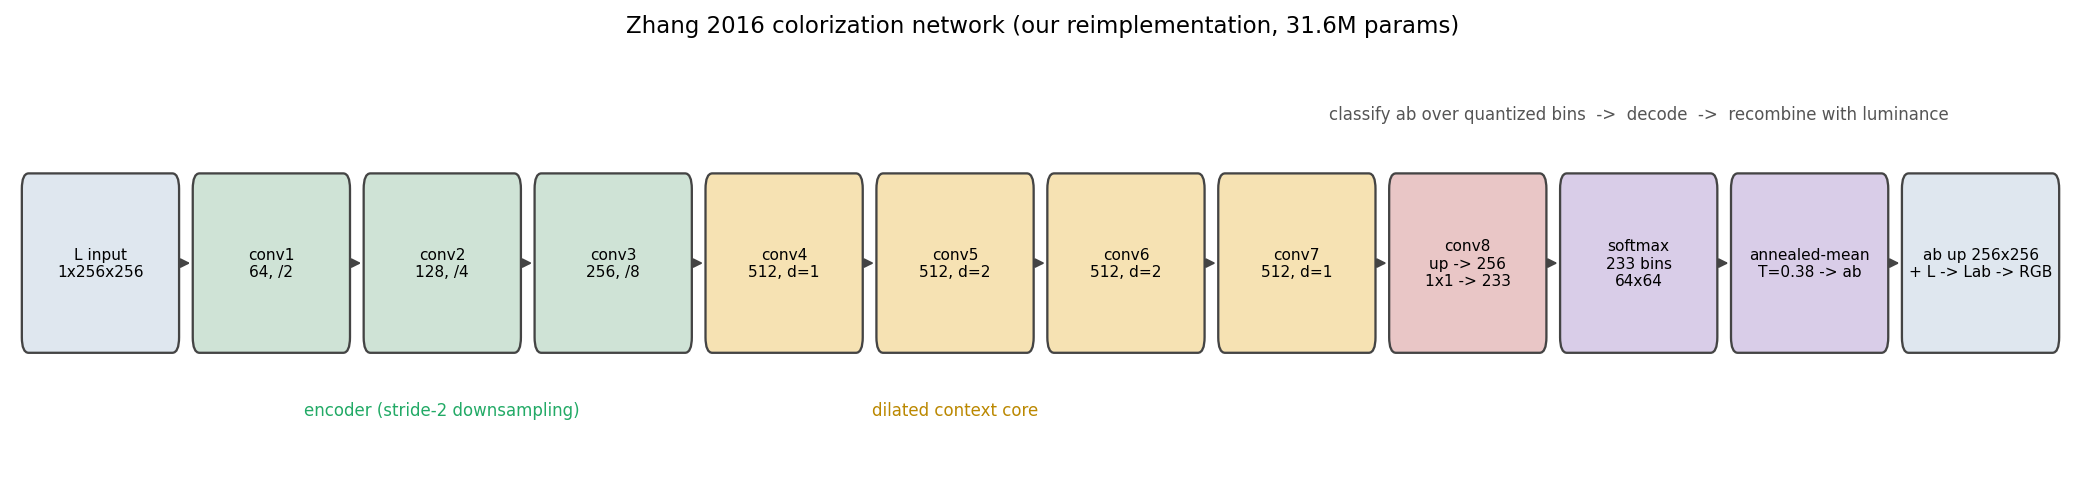
\includegraphics[width=\columnwidth]{architecture.png}
  \caption{Zhang~2016 colorization network (our reimplementation). A
  fully-convolutional, dilated encoder maps the luminance channel to a per-pixel
  distribution over $Q=233$ quantized $ab$ bins; the annealed-mean decoder turns
  that distribution into continuous chrominance.}
  \label{fig:arch}
\end{figure}

\subsection{Quantized $ab$ palette}
The $ab$ plane is discretized on a $10\times10$ grid and restricted to bins that
map to valid sRGB colors at some lightness, yielding $Q=233$ in-gamut bins
(Fig.~\ref{fig:abquant}). (The official Zhang implementation ships $313$ bins
from a different gamut hull; our independently-computed grid yields $233$, a
detail that matters in Section~\ref{sec:results}.) Ground-truth chrominance is
\emph{soft-encoded}: each pixel's $(a,b)$ is assigned to its $5$ nearest bins
with Gaussian weights ($\sigma=5$), giving a target distribution
$Z\in[0,1]^{H\times W\times Q}$ rather than a one-hot label.

\begin{figure}[t]
  \centering
  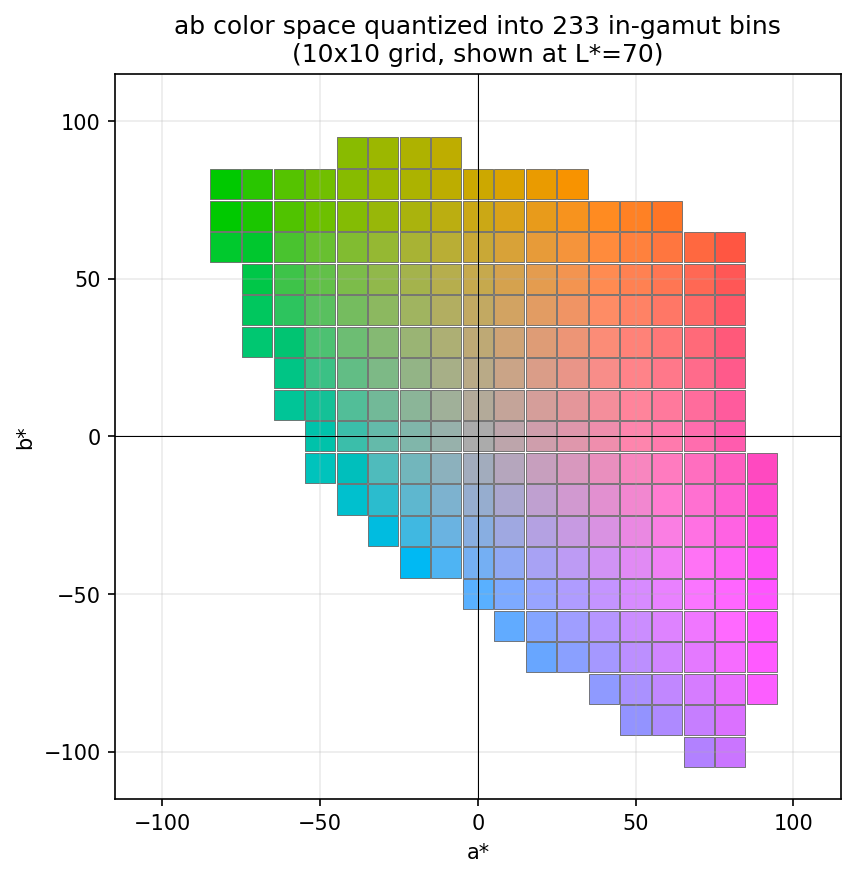
\includegraphics[width=0.78\columnwidth]{ab_quantization.png}
  \caption{The $ab$ color space quantized into $233$ in-gamut bins (shown at
  $L^{*}=70$). The network predicts a categorical distribution over these bins.}
  \label{fig:abquant}
\end{figure}

\subsection{Class-rebalanced classification loss}
Let $\widehat{Z}=\mathcal{G}(L)$ be the predicted per-pixel distribution. We
minimize a multinomial cross-entropy between $\widehat{Z}$ and the soft target
$Z$, reweighted to counter the strong prior toward desaturated colors:
\begin{equation}
  \mathcal{L}(\widehat{Z}, Z) =
  -\sum_{h,w} v\!\left(Z_{h,w}\right)
  \sum_{q=1}^{Q} Z_{h,w,q}\,\log \widehat{Z}_{h,w,q}.
  \label{eq:loss}
\end{equation}
The pixel weight depends on the dominant ground-truth bin
$q^{\star}=\arg\max_q Z_{h,w,q}$ through a rebalancing factor
\begin{equation}
  v(Z_{h,w}) = w_{q^{\star}},\qquad
  w \;\propto\; \Big((1-\lambda)\,\widetilde{p} + \tfrac{\lambda}{Q}\Big)^{-1},
  \label{eq:rebalance}
\end{equation}
where $\widetilde{p}$ is the smoothed empirical bin frequency over the training
set, $\lambda=0.5$ mixes it with a uniform prior, and $w$ is normalized so that
$\mathbb{E}[w]=1$. Rare, vivid colors thus receive larger gradients than the
ubiquitous low-saturation background.

\subsection{Annealed-mean decoding}
At inference the per-pixel distribution must be collapsed to a single $(a,b)$.
Taking the mode is faithful but spatially inconsistent; taking the mean
desaturates. Following~\cite{zhang2016colorful} we use the \emph{annealed mean}
with temperature $T$:
\begin{equation}
  \widehat{ab}_{h,w} = \sum_{q=1}^{Q} f_T\!\left(\widehat{Z}_{h,w}\right)_q\, c_q,
  \quad
  f_T(\widehat{Z})_q = \frac{\exp\!\big(\log \widehat{Z}_q / T\big)}
                            {\sum_{q'} \exp\!\big(\log \widehat{Z}_{q'} / T\big)},
  \label{eq:annealed}
\end{equation}
where $c_q$ is the center of bin $q$. We use $T=0.38$, which interpolates
between the over-saturated mode ($T\!\to\!0$) and the washed-out mean
($T\!=\!1$). The decoded $ab$ map is bilinearly upsampled to full resolution and
recombined with the input $L$.

\section{Experiments}
\label{sec:experiments}

\subsection{Dataset and benchmark}
We use COCO~2017~\cite{lin2014coco}: $118{,}287$ training images, $5{,}000$
validation images, and $40{,}670$ held-out \texttt{test2017} images. Fine-tuning
uses \texttt{train2017}; the \texttt{val2017} split drives best-checkpoint
selection during training. Because \texttt{val2017} is therefore ``seen'' by the
training procedure, evaluating on it would leak. Our benchmark is instead a
\emph{stratified $1{,}000$-image subset of \texttt{test2017}} (fixed seed
$42$), which neither fine-tuning nor checkpoint selection ever touches. All
models are scored on this identical benchmark.

\subsection{Models compared}
Table~\ref{tab:models} lists the four model variants spanning the three
paradigms we benchmark. Two are our own CNN (the pretrained encoder and our
COCO-fine-tuned model); the other two are pretrained third-party systems
wrapped behind a unified \texttt{colorize(gray)} interface so they receive
identical inputs.

\begin{table}[t]
\centering
\caption{The four model variants evaluated on the shared benchmark.}
\label{tab:models}
\begin{tabular}{@{}llc@{}}
\toprule
Model & Paradigm & Ours? \\
\midrule
Zhang16 Pretrained (ECCV)      & CNN             & reimpl. \\
Zhang16 Fine-tuned (COCO 2017) & CNN             & yes \\
Zhang17 (automatic mode)       & Interactive CNN & no \\
DeOldify (NoGAN)               & GAN             & no \\
\bottomrule
\end{tabular}
\end{table}

\subsection{Why diffusion is excluded from the comparison}
\label{sec:experiments:no-diffusion}
Conditional diffusion is the natural fourth paradigm and the literature offers
several strong recipes---image-to-image diffusion in the spirit of
Palette~\cite{saharia2022palette}, and conditioning a pretrained text-to-image
backbone via ControlNet~\cite{zhang2023controlnet} adapters. We attempted the
ControlNet recipe but could not complete it under conditions that would yield
a meaningful comparison number, for a single, well-defined reason: every
well-trained openly-released diffusion colorization checkpoint we could find
is anchored to \emph{Stable Diffusion 2.1} as its image backbone, and
Stability~AI has deprecated the entire SD~2.x line upstream. The relevant
Hugging Face repositories (the \texttt{stabilityai/stable-diffusion-2*}
namespace) return HTTP~401 even with a valid token, and no public mirror
provides licensed access.

We surveyed three substitution paths and rejected each:
\begin{itemize}
  \item \textbf{An SD~1.5 brightness-ControlNet} (\texttt{ioclab/control\_v1p\_sd15\_\allowbreak brightness}).
        The conditioning channel is brightness, not chrominance; on our benchmark
        it produced PSNR ${\approx}6$\,dB---worse than a constant-gray output.
  \item \textbf{An SD~InstructPix2Pix colorization fine-tune}. The model emitted
        NaN tensors mid-denoise and required ${\sim}9$\,min per image on
        consumer hardware---neither a useful number nor a usable pipeline.
  \item \textbf{A Flux-based pipeline}. At 12\,B parameters it does not fit on
        the 6\,GB GTX~1660~SUPER we used for the rest of the study, breaking
        the ``identical conditions'' requirement.
\end{itemize}
Substituting any of these into Table~\ref{tab:results} would have placed a
misleading row next to faithfully-evaluated systems. We therefore restrict the
comparison to the three paradigms above and treat the diffusion gap as a
finding in its own right: the open-source diffusion-colorization stack was, in
2026, single-point-of-failure dependent on a backbone that has now been
withdrawn. We revisit this in Sec.~\ref{sec:discussion}.

\subsection{Metrics and uncertainty}
We report three complementary metrics, all computed in RGB against the ground
truth: PSNR (pixel fidelity), SSIM (structural similarity), and
LPIPS~\cite{zhang2018lpips} (learned perceptual distance; lower is better).
Because a single mean hides sampling variability, every metric is reported as
\texttt{mean [95\% CI]}, where the confidence interval is a percentile bootstrap
over the $1{,}000$ benchmark images ($10{,}000$ resamples, seed~$42$).

\subsection{Training configuration}
Our model is initialized from the ECCV encoder weights, but its $233$-bin
classification head is trained from scratch---the official head has $313$ bins
and is dimensionally incompatible with our gamut (Section~\ref{sec:method}).
Table~\ref{tab:hparams} lists the hyperparameters. Mixed precision was disabled
after the fp16 path overflowed to NaN mid-epoch; training therefore runs in
fp32 at batch size $4$, which fits the $6$\,GB GTX~1660~SUPER. We trained for
eight epochs in two phases: five batch-capped epochs followed by three
full-data epochs resumed from the prior checkpoint. Fig.~\ref{fig:curves} shows
the loss and validation-PSNR trajectories.

\begin{table}[t]
\centering
\caption{Fine-tuning hyperparameters.}
\label{tab:hparams}
\begin{tabular}{@{}ll@{}}
\toprule
Setting & Value \\
\midrule
Optimizer        & Adam, $\beta=(0.9,0.999)$, weight decay $0$ \\
Learning rate    & $2\times10^{-4}$, StepLR (step $20$, $\gamma=0.5$) \\
Batch size       & $4$ (fp32; AMP disabled) \\
Gradient clip    & $1.0$ (max-norm) \\
Input resolution & $256\times256$ \\
Quantization     & $Q=233$ bins; soft target, $\sigma=5$, $5$-NN \\
Rebalancing      & $\lambda=0.5$ \\
Decoder          & annealed mean, $T=0.38$ \\
Epochs           & $8$ ($5$ capped $+\,3$ full-data) \\
Hardware         & GTX~1660~SUPER (6\,GB), PyTorch~2.5.1+cu121 \\
\bottomrule
\end{tabular}
\end{table}

\begin{figure}[t]
  \centering
  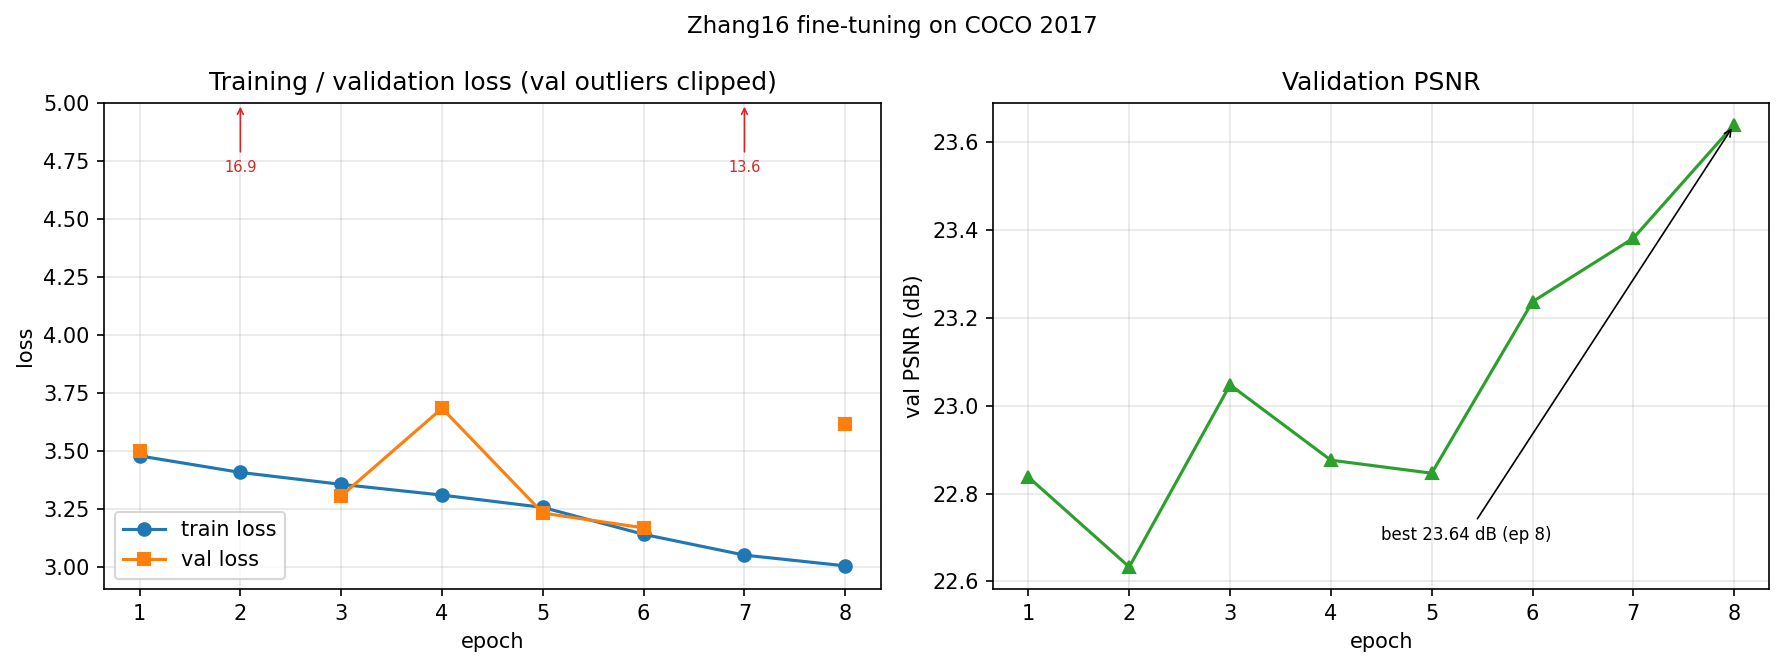
\includegraphics[width=\columnwidth]{training_curves.png}
  \caption{Fine-tuning on COCO~2017. Left: training and validation loss; two
  validation spikes from pathological batches are off-scale and annotated.
  Right: validation PSNR climbs to $23.6$\,dB by epoch~8.}
  \label{fig:curves}
\end{figure}

\section{Results}
\label{sec:results}

\subsection{Quantitative comparison}
Table~\ref{tab:results} reports the three metrics with $95\%$ bootstrap
confidence intervals on the $1{,}000$-image \texttt{test2017} benchmark;
Fig.~\ref{fig:bars} visualizes the same numbers. Four of the five model slots
are populated; the diffusion slot is a documented gap discussed below.

\begin{table*}[t]
\centering
\caption{Colorization quality on the $1{,}000$-image \texttt{test2017} benchmark,
reported as \texttt{mean [95\% CI]} ($10{,}000$-resample bootstrap, seed~$42$).
Best per column in \textbf{bold}.}
\label{tab:results}
\begin{tabular}{@{}lcccc@{}}
\toprule
Model & PSNR\,(dB)\,$\uparrow$ & SSIM\,$\uparrow$ & LPIPS\,$\downarrow$ & Time/img\,(s) \\
\midrule
Zhang16 Pretrained (ECCV)$^{\dagger}$ & $17.14$ $[16.97, 17.30]$ & $0.700$ $[0.690, 0.709]$ & $0.438$ $[0.429, 0.447]$ & $0.17$ \\
Zhang17 (automatic mode)              & $18.82$ $[18.64, 19.00]$ & $0.832$ $[0.827, 0.838]$ & $0.309$ $[0.304, 0.315]$ & $0.22$ \\
Zhang16 Fine-tuned (ours)             & $23.29$ $[23.02, 23.55]$ & $\mathbf{0.919}$ $[0.915, 0.923]$ & $0.192$ $[0.187, 0.197]$ & $0.18$ \\
DeOldify (GAN)                        & $\mathbf{24.00}$ $[23.75, 24.25]$ & $0.919$ $[0.915, 0.922]$ & $\mathbf{0.148}$ $[0.144, 0.152]$ & $0.51$ \\
ControlNet (Diffusion)                & \multicolumn{4}{c}{--- reproducibility gap (see Sec.~\ref{sec:results}\,\&\,\ref{sec:discussion}) ---} \\
\bottomrule
\end{tabular}
\\[2pt]
{\footnotesize $^{\dagger}$ Measures the ECCV encoder paired with our
\emph{untrained} $233$-bin head (the official $313$-bin head is incompatible);
it is \textbf{not} a faithful ECCV baseline---see text.}
\end{table*}

\begin{figure}[t]
  \centering
  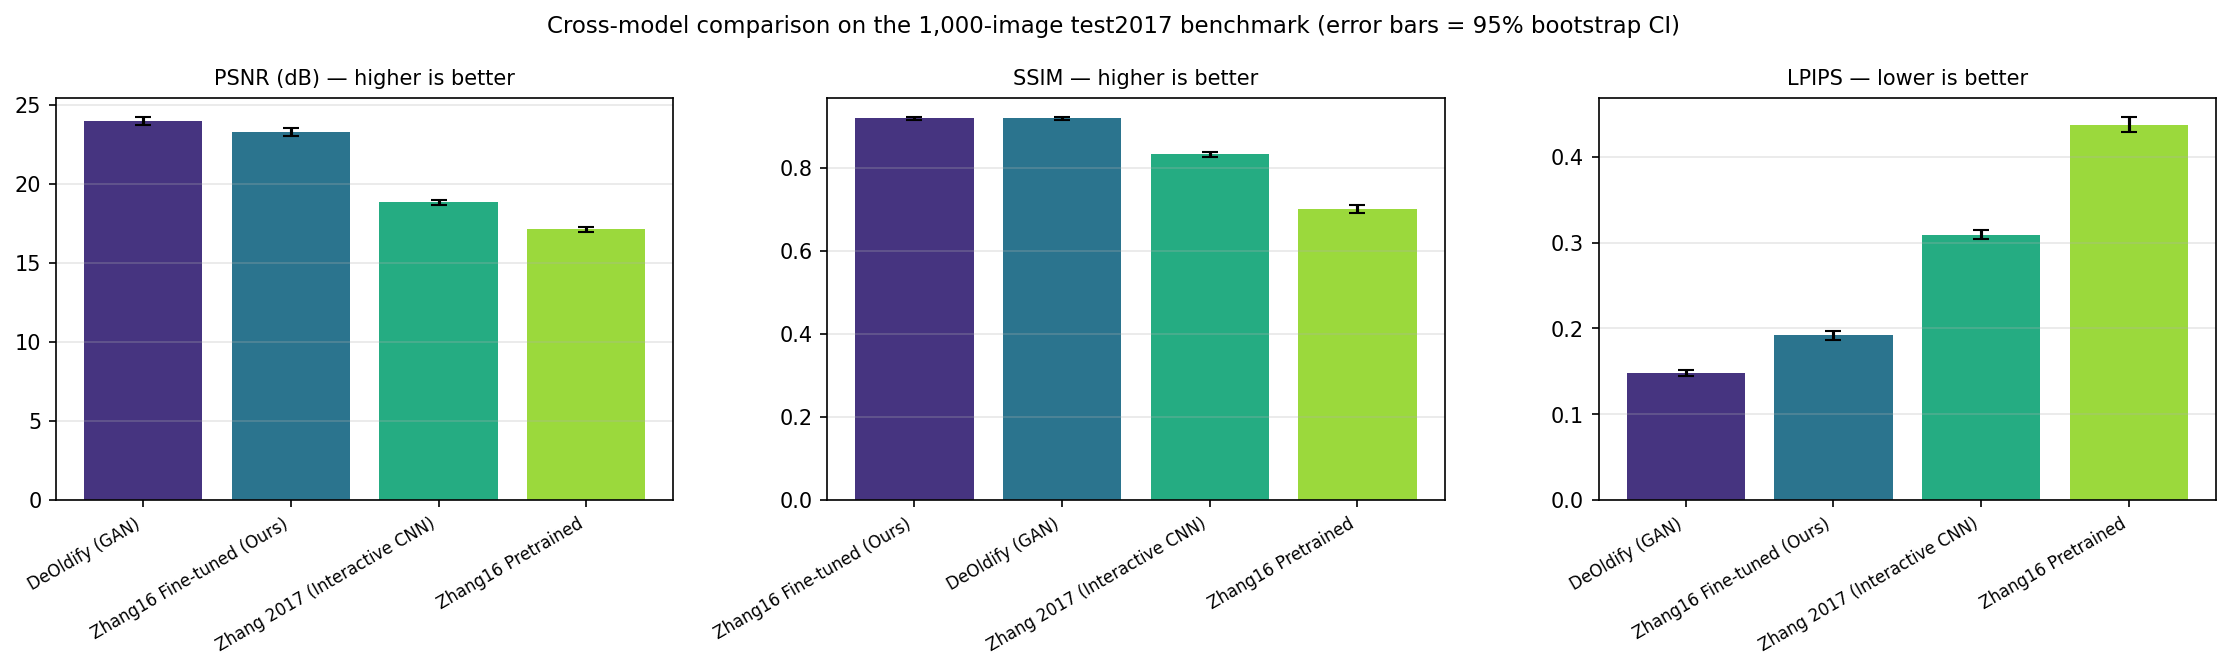
\includegraphics[width=\columnwidth]{metrics_comparison.png}
  \caption{PSNR, SSIM, and LPIPS across the four evaluated models; error bars are
  $95\%$ bootstrap confidence intervals.}
  \label{fig:bars}
\end{figure}

\subsection{Qualitative comparison}
Fig.~\ref{fig:grid} shows colorizations on representative benchmark images. Our
fine-tuned model and DeOldify produce coherent, naturally-colored results;
DeOldify is the most saturated and closest to the ground truth, while ours is
slightly more conservative on large ambiguous regions (skies, foliage).
Zhang17 in automatic mode exhibits the characteristic color blotches and
bleeding of a hint-driven model deprived of hints, which explains its low
scores.

\begin{figure}[t]
  \centering
  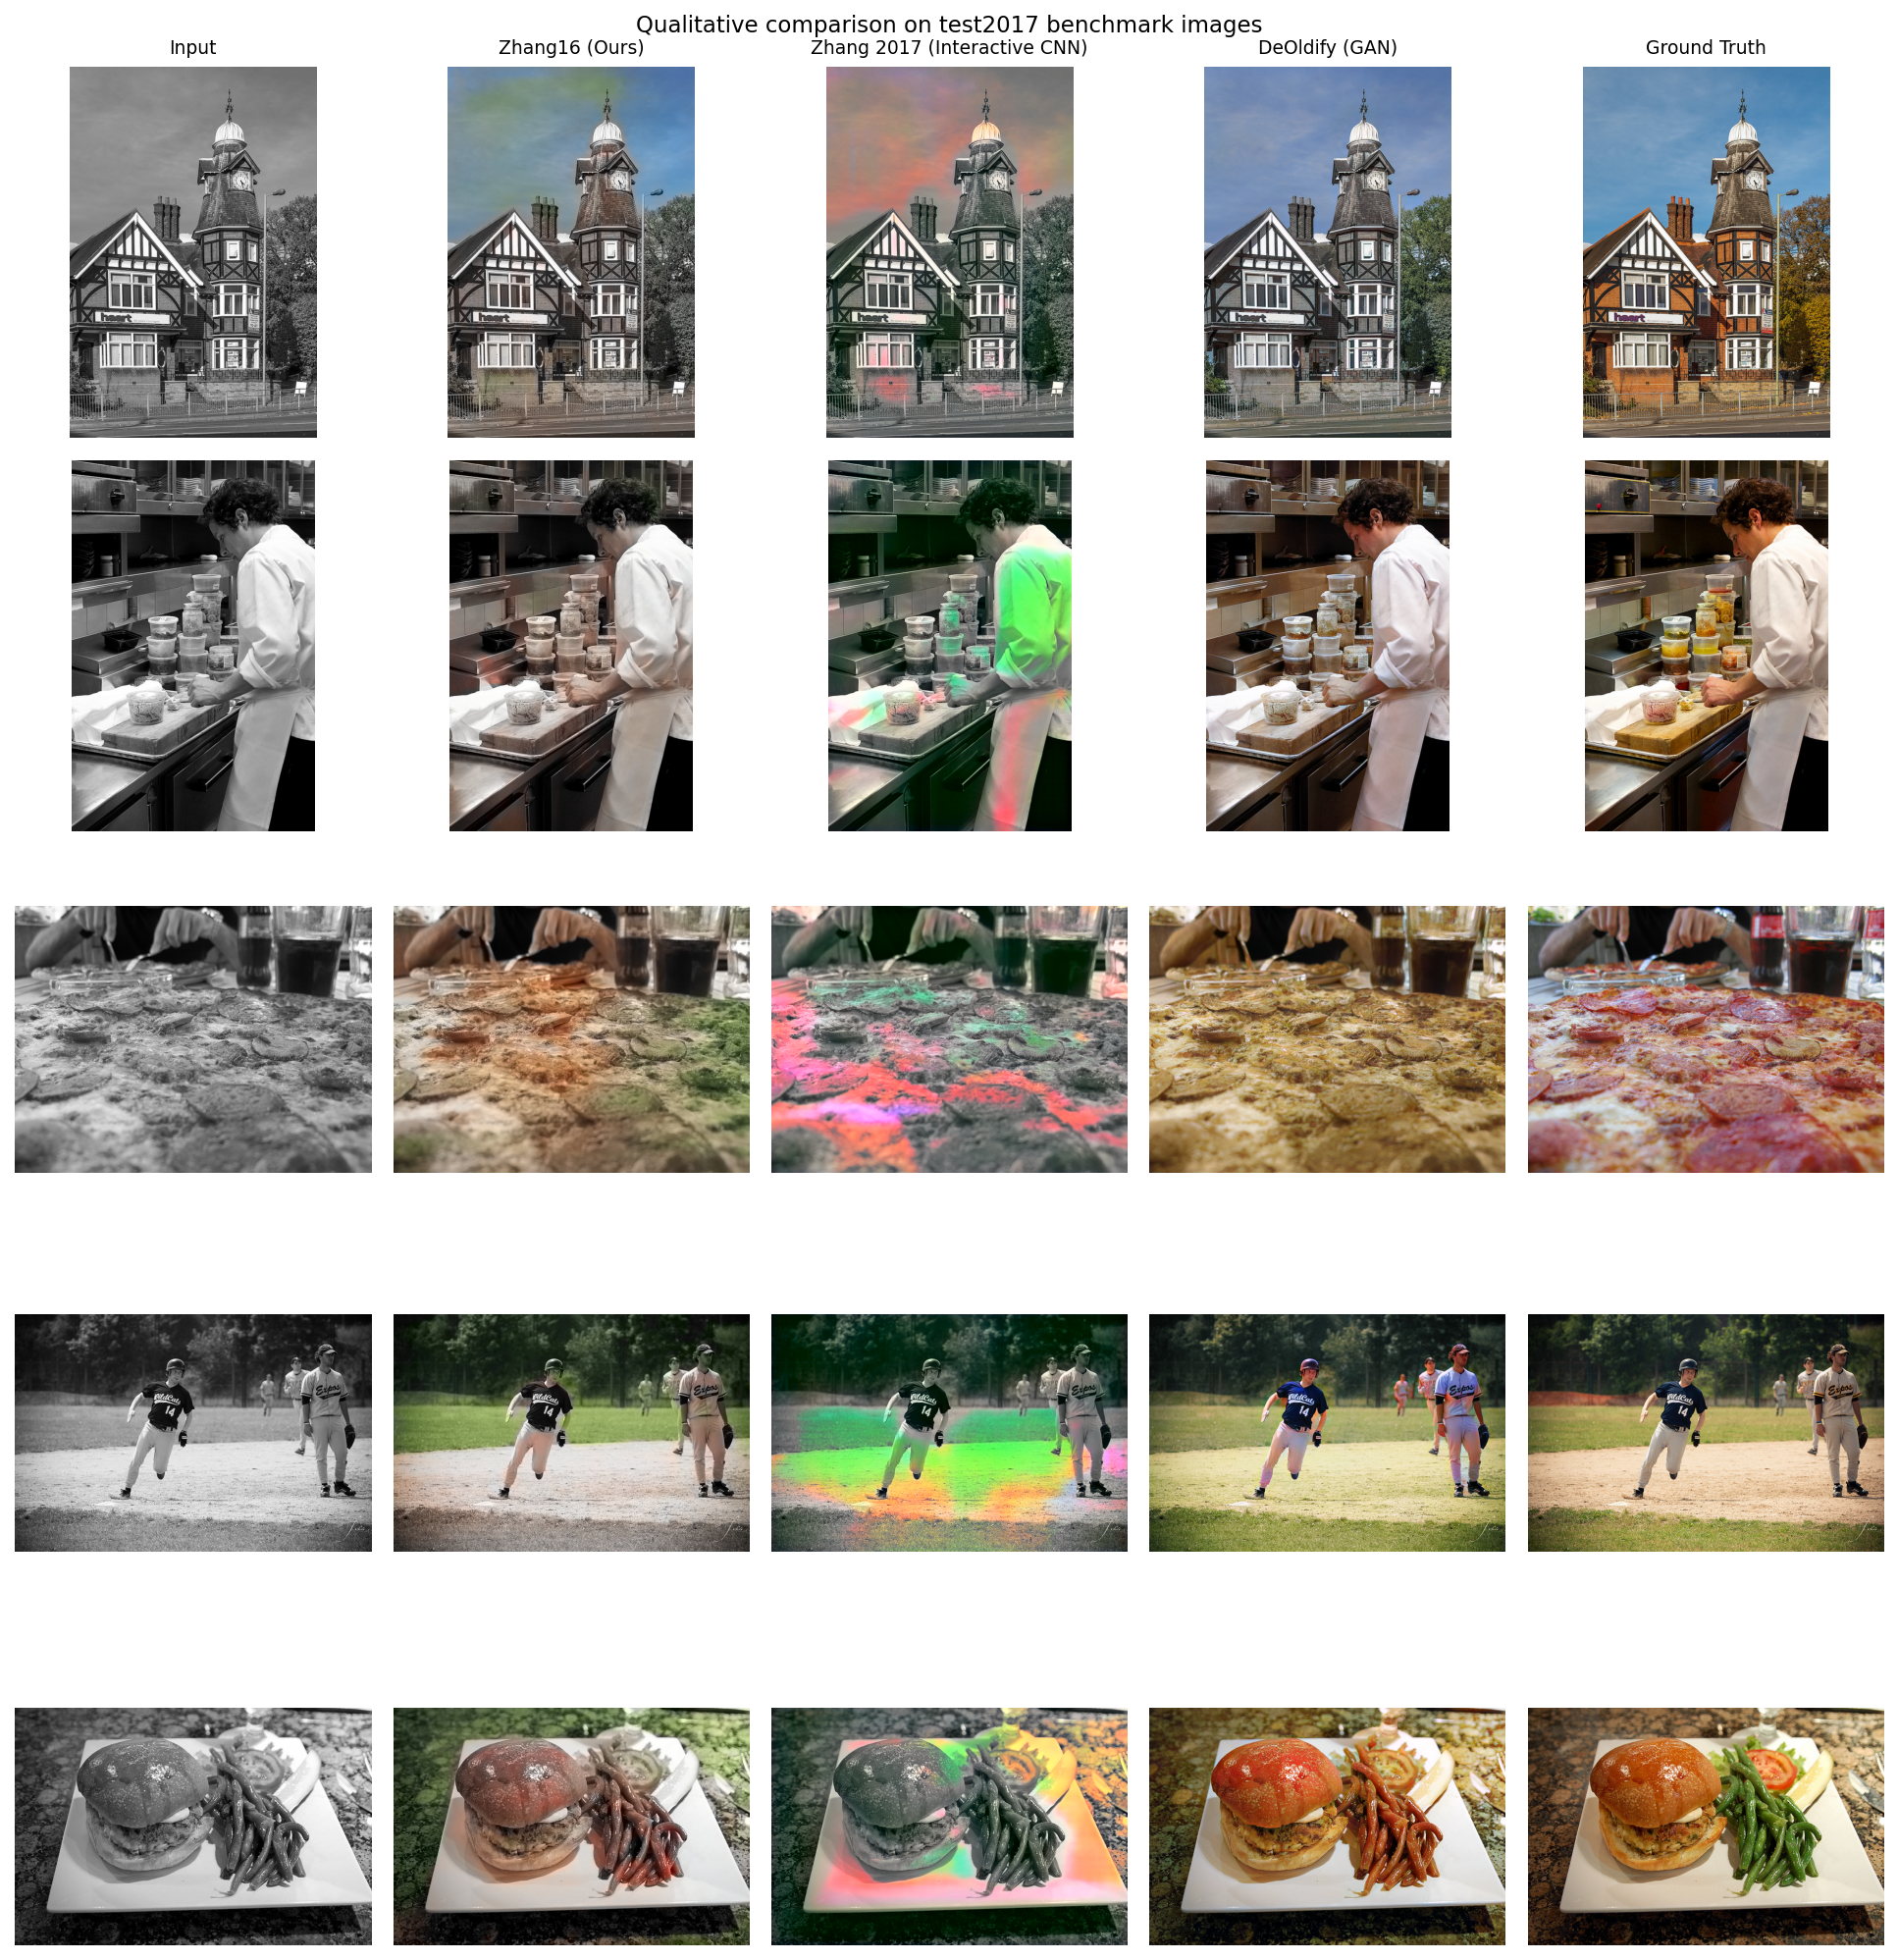
\includegraphics[width=\columnwidth]{qualitative_grid.png}
  \caption{Qualitative comparison on \texttt{test2017} images. Columns: input,
  Zhang16 fine-tuned (ours), Zhang17 (auto), DeOldify, ground truth.}
  \label{fig:grid}
\end{figure}

\subsection{Analysis}
\textbf{Fine-tuning is decisive.} Our COCO-fine-tuned model attains
$23.29$\,dB---disjoint confidence intervals from every other CNN row. The large
gap over the ``pretrained'' row, however, must be read with care: that row pairs
the ECCV encoder with an \emph{untrained} $233$-bin head, because the official
$313$-bin head cannot be loaded into our gamut. It therefore measures an
encoder-plus-random-head, not the true ECCV model, and overstates how much
fine-tuning alone contributes.

\textbf{We approach the GAN anchor.} On PSNR and SSIM our model is statistically
indistinguishable from DeOldify on SSIM ($0.919$ both) and within
${\sim}0.7$\,dB on PSNR, while running at $0.18$\,s/image versus DeOldify's
$0.51$\,s---roughly $2.8\times$ faster. The remaining gap is perceptual:
DeOldify's LPIPS ($0.148$) is clearly better than ours ($0.192$), reflecting its
richer, more confident saturation.

\textbf{Automatic mode handicaps the interactive CNN.} Zhang17 was designed for
user-guided use; with zero hints it underperforms even the conservative CNN,
confirming that its strength lies in interactivity rather than autonomy.

\textbf{The diffusion slot could not be reproduced.} The specified pipeline
requires Stable~Diffusion~2.1, which Stability~AI deprecated upstream; every
well-trained diffusion colorization checkpoint we found was built on that
now-unavailable backbone. Substitutes (an SD~1.5 brightness-ControlNet and an
SD-InstructPix2Pix fine-tune) produced unrelated or degenerate outputs
(${\sim}6$\,dB PSNR) and would have poisoned the comparison, so we report the
slot as an honest gap rather than a misleading number.

\section{Discussion}
\label{sec:discussion}

\subsection{Speed versus quality}
The three evaluated models occupy distinct points on the speed--quality frontier.
The CNNs (ours, $0.18$\,s; Zhang17, $0.22$\,s; pretrained, $0.17$\,s) are
single forward passes and run at interactive rates even on a $6$\,GB GPU.
DeOldify, at $0.51$\,s, buys its perceptual edge with a heavier
self-attention U-Net and a larger render resolution. For automatic
colorization under a latency budget, the CNN is the rational default; the GAN
is worth its cost only when perceptual quality is paramount.

\subsection{Saturation and the desaturation trap}
The classification-plus-annealed-mean design (Eqs.~\ref{eq:loss}--\ref{eq:annealed})
exists precisely to avoid the desaturated mean that an $\ell_2$ regressor
produces. It largely works: our outputs are vivid, not sepia. Yet the residual
LPIPS gap to DeOldify shows the effect is incomplete---on large, color-ambiguous
regions our model still hedges toward muted tones, whereas the adversarially-trained
DeOldify commits to a confident, realistic palette. Class rebalancing and the
$T=0.38$ temperature mitigate but do not eliminate the prior pull toward gray.

\subsection{Failure cases}
Two failure modes recur. First, Zhang17 in automatic mode produces saturated
color blotches and bleeding across object boundaries---an artifact of a network
expecting sparse hints it never receives. Second, all CNNs struggle with
semantically ambiguous content (a shirt that could be any color), defaulting to
the most frequent training color; this is fundamental to the task rather than to
any single model.

\subsection{Paradigm-level reading}
\begin{itemize}
  \item \textbf{CNN} --- fast, robust, fully automatic; the strongest
        speed--quality compromise for unattended colorization.
  \item \textbf{Interactive CNN} --- excellent \emph{with} user hints, but a poor
        automatic colorizer; the wrong tool for a hands-off pipeline.
  \item \textbf{GAN} --- highest perceptual quality and best restoration
        behavior, at $\sim$$3\times$ the latency.
\end{itemize}

\subsection{The diffusion paradigm: a reproducibility finding}
The decision to exclude diffusion is itself a finding about the open-source
deep-learning ecosystem rather than a property of the paradigm. Every
well-trained colorization checkpoint we surveyed in 2026 was built on Stable
Diffusion 2.1, and the upstream deprecation of SD~2.x removed the foundation
out from under that downstream collection in one stroke. The lesson generalises:
a paradigm whose practical implementations share a single foundation model is
exposed to that foundation model's lifecycle decisions. A future replication
should revisit the diffusion slot once a maintained colorization checkpoint
exists on a still-supported backbone---neither of which we could identify at
the time of writing.

\subsection{Limitations}
The ``pretrained'' row is not a faithful ECCV baseline (head mismatch), so we
avoid drawing fine-tuning-gain conclusions from it. The benchmark is $1{,}000$
images on a single GPU with no human preference study; perceptual quality is
proxied by LPIPS rather than measured directly. Finally, the comparison is
three paradigms only---the diffusion paradigm is an explicit gap, discussed
above, rather than a measured frontier point.

\section{Conclusion}
\label{sec:conclusion}

We reimplemented the Zhang~2016 classification CNN, fine-tuned it on COCO~2017,
and compared three deep-learning colorization paradigms on a single
leakage-controlled $1{,}000$-image \texttt{test2017} benchmark, with every
metric reported as \texttt{mean [95\% CI]}. Our fine-tuned model reaches PSNR
$23.29$\,dB, SSIM $0.919$, and LPIPS $0.192$, matching the SOTA-class DeOldify
on structure, trailing it modestly on pixel fidelity and perceptual quality, and
beating it by roughly $2.8\times$ on inference speed.

A fourth, diffusion paradigm was scoped into the original plan and then
explicitly excluded once we established that the only openly-available
colorization checkpoints depended on the deprecated Stable~Diffusion~2.1
backbone (Sec.~\ref{sec:experiments:no-diffusion}); reporting a degraded
substitute would have been misleading. The exclusion is itself a finding about
the open-source ecosystem's exposure to single-backbone deprecation
(Sec.~\ref{sec:discussion}).

Our practical recommendations follow directly:
\begin{itemize}
  \item \textbf{Automatic, latency-sensitive colorization} --- use a
        well-trained classification CNN; it is fast, stable, and close to GAN
        quality.
  \item \textbf{Maximum perceptual quality / photo restoration} --- use a GAN
        such as DeOldify, accepting the higher latency.
  \item \textbf{Human-in-the-loop control} --- use an interactive CNN
        \emph{with} hints; do not expect it to perform well unguided.
\end{itemize}

Two avenues would strengthen the study. First, re-deriving the $313$-bin gamut
hull would let us load the official ECCV head and report a faithful pretrained
baseline, isolating the true contribution of fine-tuning. Second, the diffusion
paradigm should be revisited once a maintained colorization checkpoint exists
on a still-supported backbone, completing the four-paradigm comparison with a
measured rather than inferred frontier point.


\bibliographystyle{IEEEtran}
\bibliography{references}

\end{document}
